\documentclass{article}
\usepackage[utf8]{inputenc}
\usepackage[
  colorlinks=true,
  urlcolor=blue
]{hyperref}
\usepackage{amsmath}
\usepackage{xcolor,colortbl}
\definecolor{Amber}{rgb}{1.0, 0.75, 0.0}
\definecolor{LightCyan}{rgb}{0.88,1,1}

\newcolumntype{a}{>{\columncolor{LightCyan}}c}
\newcolumntype{b}{>{\columncolor{Amber}}c}

% for affiliation
\usepackage{authblk}
\usepackage{textcomp}
\usepackage{stackengine,graphicx}
\newcommand\No[1][.13ex]{%
  \setbox0=\hbox{\scalebox{.7}{o}}%
  \setbox2=\hbox{N}%
  N\kern-.05em\stackengine{\dimexpr\ht0-\ht2+#1}{\belowbaseline[-\ht2]{\copy0}}%
    {\rule[-.13ex]{.7\wd0}{.13ex}}%
    {U}{c}{F}{F}{L}%
}
% for histograms
\usepackage{tikz}
\usepackage{pgfplots}
\usepackage{float}
\pgfplotsset{width=7.5cm,compat=1.12}
\usepgfplotslibrary{fillbetween}


\title{Natural Language Processing\\Phase \No3: Final}
\date{July 2021}
\author{Pooya Kabiri}
\affil{Department of Computer Science}
\affil{Iran University of Science and Technology}

\begin{document}

\maketitle

{
\hypersetup{linkcolor=black}
\tableofcontents
\listoffigures
\addcontentsline{toc}{section}{\listfigurename}
}
\pagebreak

\section{Word2Vec}
\par I used A2 code on two class of my data which are chandler and phoebe.
\par I changed the code for StanfordSentiment Dataset and turned it into FriendsDataset which I could use with my own data. I trained a word2vec model for each class, each for 5000 iterations, and saved the final models as requested.

\par For every common word between the two classes I computed a cosine similarity, which was 2640 common words, every 20 of them in a single report photo.

\begin{figure}[H]
    \centering
    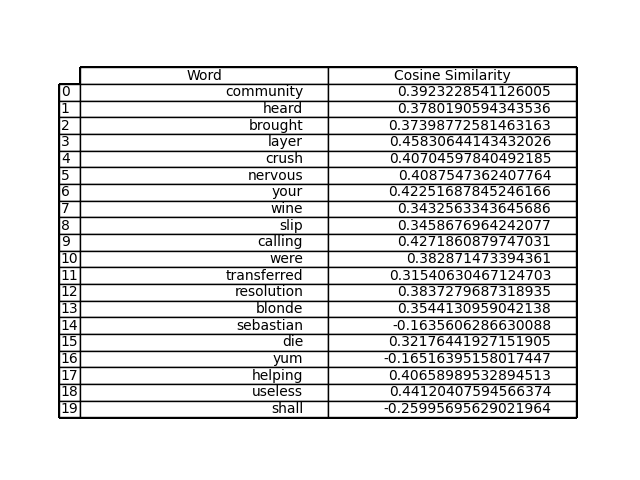
\includegraphics[width=1\linewidth]{../reports/word2vec/common_words_122.png}
    \caption{Cosine Similarity}
\end{figure}

\par For example in this photo, the word 'yum' has a low similarity, and I think that because Phoebe is a very sarcastic person and usually uses the word 'yum' in a sarcastic way, meaning the opposite (not delicious), but chandler is not sarcastic and loves food, so that's maybe why the similarity in the context of the dialogues very low.

\par In this photo, the word 'Janice' has a high sim score, they both hate her character and usually everything stated about Janice is negative by the both of them. They both hate her so much. I can think of this as a reason that maybe Janice has a high sim score in both characters' context.\\

\par There are 132 report pictures under \texttt{reports/word2vec/} and it contains sim score for all common vocabulary.

\section{Tokenization}
\par for this section I used SentencePiece module as requested, and trained data for each 2 labels separately.
\par On each training procedure, 0.2 of the data is used for testing and counting the number of predicted unk tokens.
\par the maximum number for vocabulary which the framework allowed me to use was 11737.

\begin{figure}[H]
    \centering
    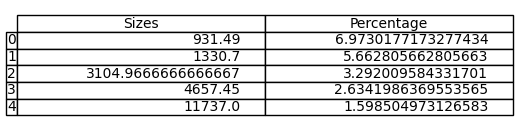
\includegraphics[width=\inewidth]{../reports/tokenization/percentages.png}
    \caption{unk percent, for vocab size}
\end{figure}

\par As seen from the table, the more the vocab size, the tokenizer performs better and the percentage of unk tokens is smaller. Best result is from the maximum possible size of vocab (11737) , which is 1.59\%, and also the size is not too big and it can be used without any size problems. This model is copied under \texttt{models/tokenization} as the best model.\footnote{\href{https://colab.research.google.com/github/google/sentencepiece/blob/master/python/sentencepiece_python_module_example.ipynb#scrollTo=ee9W6wGnVteW}{Used resource}}

\section{Dependency Parsing}

\par For this part I used A3 code, trained it on the assignment's train data. I manually parsed 10 sentences from my data using Conllu editor, I did POS tagging and Dependency Parsing on them, and then fed them into the neural network as test data. I got a UAS score of 76.42\% on these 10 sentences.

\par The annotated file for 10 test sentences can be found under \texttt{data/parsing}.\\

\par Example \No1:

\textbf{My erection is back !}\\

\par UAS score for this example : 0.5

\par The model has chosen 'erection' as the root, but it is false. The head for 'erection' is 'is', but the model has predicted it the other way.\\\\

\par Example \No2:

\textbf{I learned never to borrow money from friends .}\\

\par UAS score for this example : 0.875, which is pretty good.

\par The model has chosen 'learned' for the head of 'never', instead of the correct dependency which is that 'borrow' is the correct head for 'never'. In this case I think because 'never' is an adverb and there are two verb phrases in the sentence, it is hard to predict that this adverb describes which of the verbs.\\\\

\par Example \No3:

\textbf{I tend to keep talking until somebody stops me
.}\\

\par UAS score for this example : 0.88, which is also decent.

\par The model only predicted one dependency wrong, which is the head of 'stops'. Model prediction is 'tend', but the correct head is 'keep'. The model didn't predict that this adverb clause belongs to which verb.\\\\

\par Example \No4›:

\textbf{My idea of a vacation does not involve spmething sucking on my nipples until they are raw .}\\

\par UAS score for this example : 1.0

\par The model predicted this long sentence fully correctly. It is a funny, informal sentence but the model predicted all of the dependencies correctly, resulting in a score of UAS 1.0. (Sorry for the adult language :D).


\section{Language Model}
\par For this section I used a code from the provided source. The model is a LSTM with 3 layers, hidden state size of 128, and also embedding size of 128, followed by a dropout layer (p=0.2).

\par the data fed to this network is cleaned using stopword and contradiction removal and tokenization. 

\par I used the two models to generate sentences providing the model a single starting word. the full results are under \texttt{reports/language\_model}.\\\\\\

\begin{center}
\begin{tabular}{ |c|c| } 
 \hline
 coffee spade the plate in up out guitar . so i & Phoebe  \\ 
 \hline
 coffee sooner laughs tomorrow , but uh beam look you said & Chandler  \\ 
 \hline
\end{tabular}
\end{center}

\begin{center}
\begin{tabular}{ |c|c| } 
 \hline
 smelly focusing . how just i m , and very coffee & Phoebe  \\ 
 \hline
 smelly battling piece open feels time we do ? i know & Chandler  \\ 
 \hline
\end{tabular}
\end{center}

\begin{center}
\begin{tabular}{ |c|c| } 
 \hline
 monica dolls jerks spray him . hi ! it s me & Phoebe  \\ 
 \hline
 monica just chicken kind than individual vaporizing teach you the in & Chandler  \\ 
 \hline
\end{tabular}
\end{center}

\begin{center}
\begin{tabular}{ |c|c| } 
 \hline
 joey smoke got lessons one . because , and cool . & Phoebe  \\ 
 \hline
 joey rehearse ! thanks there interview ? yes , i think & Chandler  \\ 
 \hline
\end{tabular}
\end{center}

\begin{center}
\begin{tabular}{ |c|c| } 
 \hline
 home latour base room ? because because you just get us & Phoebe  \\ 
 \hline
 home howie staying , take this then  . and & Chandler \\ 
 \hline
\end{tabular}
\end{center}

\par The result are not satisfying, but I can see some very little changes in the generated texts. Phoebe usually speaks in a very word-by-word way and uses very short sentences.\footnote{\href{https://www.kdnuggets.com/2020/07/pytorch-lstm-text-generation-tutorial.html}{Used Code}}


\section{Fine-Tuning}

\par For this section, I used a code from HuggingFace which is provided in the footnote. It used a model checkpoint of distil GBT2 for 'casual language modeling' task. I used this pretrained model to fine tune two labels of my data, which are chandler and phoebe, as before.

\par I splitted the data in a 80-20 way for train and dev sets. I trained the model for 5 epochs.\\

\par The perplexity for each class:

\begin{center}
\begin{tabular}{ |c|c| } 
 \hline
 Chandler & 43.57  \\ 
 \hline
 Phoebe & 40.59 \\ 
 \hline
\end{tabular}
\end{center}

\par Now, I used the same start words as the section 4 for text generation. Here are the results:

\begin{center}
\begin{tabular}{ |c|c| } 
 \hline
 coffee !um , so , are you listening ?oh , how is it ?really ?no & Phoebe  \\ 
 \hline
 coffee and honey , he gave us .we have you all  together in this apartment !they & Chandler  \\ 
 \hline
\end{tabular}
\end{center}

\begin{center}
\begin{tabular}{ |c|c| } 
 \hline
 smelly and the man !hey !why mma mike mike , i know !hey & Phoebe  \\ 
 \hline
 smelly !good bye mary !oh hey , i'm .well , this is what i & Chandler  \\ 
 \hline
\end{tabular}
\end{center}


\begin{center}
\begin{tabular}{ |c|c| } 
 \hline
 monica , it would be great !oh !yeah :no ?i am still here ;so & Phoebe  \\ 
 \hline
 monica : that  i said .look what , i am here .it sucks to have & Chandler  \\ 
 \hline
\end{tabular}
\end{center}

\begin{center}
\begin{tabular}{ |c|c| } 
 \hline
 joey , well yeah .i love you !she can take in food she knows .i & Phoebe  \\ 
 \hline
 joey !i never got into sex with her .i just wanted to get in the way & Chandler  \\ 
 \hline
\end{tabular}
\end{center}

\begin{center}
\begin{tabular}{ |c|c| } 
 \hline
 home was there ?she has to make that happen .but then we have to say we don t & Phoebe  \\ 
 \hline
 home aww , they can get everything .did that .oh hey , now i should do this & Chandler \\ 
 \hline
\end{tabular}
\end{center}

\par The results are much better improved in contrast to section 4. The sentence are correct and meaningful, just the combination of them doesn't make sense, but each sentence has a better overall structure. \footnote{\href{https://colab.research.google.com/github/huggingface/notebooks/blob/master/examples/language_modeling.ipynb}{Used Code}}\\

\par Due to Github Limitations, I uploaded my final models on Google Drive, and you can access it \href{https://drive.google.com/drive/folders/1xT46pVDgnjKds5NsGvAQKsCefXTYA6rZ?usp=sharing}{here}.
\end{document}
